\documentclass[a4paper, 12pt]{article}

\usepackage[english]{babel}
\usepackage[utf8]{inputenc}
\usepackage{amsmath}
\usepackage{textcomp}
\usepackage{gensymb}
\usepackage{graphicx}
\usepackage{booktabs}
\usepackage[colorinlistoftodos]{todonotes}
\usepackage[left=2cm,right=2cm,top=2cm,bottom=2cm]{geometry}
\usepackage{comment}
\usepackage{multirow}
\usepackage{fancyhdr}
\usepackage[font=scriptsize,labelfont=bf]{caption}
\usepackage{wrapfig}
\usepackage{titlesec}
\usepackage{natbib}
\usepackage{setspace}

\definecolor{darkgray}{rgb}{0.3,0.3,0.3}

\pagestyle{fancy}
\fancyhf{}
\fancyhead[R]{
\includegraphics[scale = 0.07]{Logo_EPFL.png}}
\fancyhead[L]{\textcolor{darkgray}{Air Pollution \& Climate Change : Assignment 1}}
\fancyfoot[R]{\textcolor{darkgray}{\thepage}}
\fancyfoot[L]{\textcolor{darkgray}{Nikolai Orgland \& Antoine Spahr}}
 
\renewcommand{\headrulewidth}{0.5pt}
\renewcommand{\footrulewidth}{0.5pt}
\renewcommand{\familydefault}{\sfdefault}
 
\titleformat{\section}
 			{\large\bfseries\sffamily}
  			{\thesection}{1em}{}
\titleformat{\subsection}
 			{\small\bfseries\sffamily}
  			{\thesubsection}{1em}{}
\titleformat{\subsubsection}
 			{\small\slshape\sffamily}
			{\thesubsubsection}{1em}{}

\begin{document}
%------------------------------- Title Page ---------------------------------------
\thispagestyle{empty}
\begin{center}
    {\large ENV-400 Air Pollution and Climate Change}\\[0.2cm]
    
    {\normalsize Spring Semester 2019 }\\[1.2cm]
    
    \hrulefill 
    \\[0.5cm]
        {\Huge\textbf{Comparative analysis of air pollutants between Sion and Tänikon}}
    \\[0.5cm]
    \hrulefill 	
\end{center}

~\\[1.3cm]

\begin{center}
    
\includegraphics[scale=0.20]{Logo_EPFL.png}\\[1.5cm]
    {\large \today}\\[0.5cm]
\end{center}

~\\[2.3cm]

\begin{centering}
    \large
    Assignment Part 1 \\
\end{centering}

~\\[1.3cm]

\begin{centering}
    \large
    Nikolai \textsc{Orgland} \textit{\small nikolai.orgland@epfl.ch}\\ 
    Antoine \textsc{Spahr} \textit{\small antoine.spahr@epfl.ch}\\
\end{centering}

\vfill
\thispagestyle{empty} 

\pagenumbering{gobble}

%---------------------------------- Table of content -----------------------------
\newpage
\tableofcontents
\pagenumbering{gobble}
\newpage
\pagenumbering{arabic}
\setcounter{page}{1}

%------------------------------ text ----------------------------------------------

\section{Introduction}
    % Present the data analysis work : 
    % -> Locations studied : Sion and Tanikon
    % -> Location properties : Sion = On Highway + bottom of valley ; Tanikon = countryside
    % -> scope of current analysis : Descriptive analysis + potential Legal limit overpass on 2018
    % -> Present which pollutant are measured : O3, NO2, NOx, PM10
    % -> Present which meteorological parameters are measured : Temperature, Precipitation, Radiation, Wind direction / wind speed

    This work analysed the air pollution data from two measurement stations in Switzerland. From these two stations, the data for the pollutants O3, NO2, NOx, PM10 as well as the meteorological parameters temperature, precipitation, radiation, wind direction/speed were collected. This data was then subject to a descriptive analysis which especially focused on the temporal evolution of the pollutants/parameters on a daily and seasonal basis. Finally, the obtained data were compared to legal limits in Switzerland for the different pollutants.
    \\
    \\
    The first station is located in Täniko in the Canton of Thurgau at 583 meters above sea level in the North-Eastern part of Switzerland. The neighbouring area is rural with small villages and characterized by strongly fertilized grassland for cattle . The closest highway is located 4 km away from the station (See Figure \ref{location_fig} b)).  
    \\
    \\
    The second station is located in Sion, the capital of the Canton of Valais in Southern Switzerland. The station is located on the military airfield of Sion at 483 meters above sea level, about 2 km south-west of the city centre. Only 50 meters away, the highway A9 passes by the station with 35’000 cars per day. The station is furthermore located in the valley of the Rhône which lies in the heart of the Swiss Alps (see Figure \ref{location_fig} a)). 
    
    \begin{figure}[h]
        \centering
        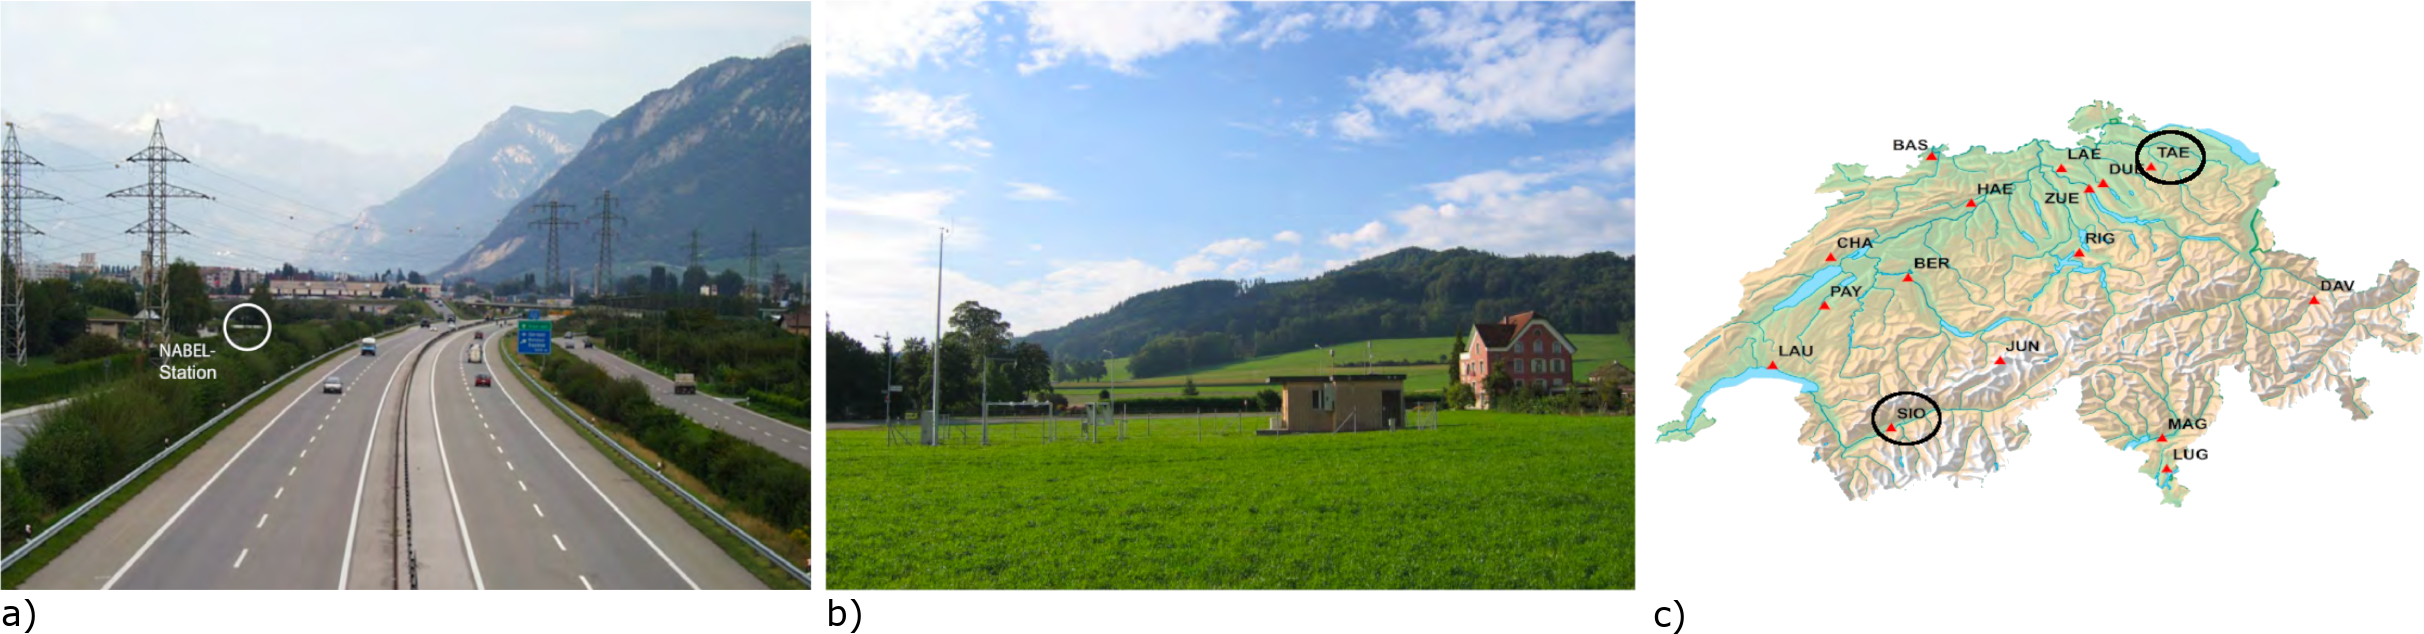
\includegraphics[width = 1 \textwidth]{Figures/Locations.png}
        \caption{\textbf{Measurement sites description.} Picture a) and b) respectively show the measurement site of Sion and Tänikon. Map c) shows the geographical situation of those two measurement stations (SIO and TAE) in Switzerland. They are highlighted with black circles. Source : \cite{NABEL}}
        \label{location_fig}
    \end{figure}

\section{Measurement Tools}
    % Present how the data for pollutant used were collected : (this section is a sort of method section)
    % -> Physical principle of the measure 
    % -> Sampling rate 
    % -> need for calibration?
    % -> precision of the measure if known 
    % -> describe the potential biases/error
    
    % in situ measurement (not satellite)
    % 
    Before performing the data analysis, the current section explains how the concentrations of the pollutants are measured at the two stations that are part of the National Air Pollution Monitoring Network (NABEL) of the Swiss Federal Office for the Environment. \cite{NABEL}
    
    \subsection{NO\textsubscript{2}, NO\textsubscript{x}}
    
        Both NO and NO\textsubscript{x} are measured by chemiluminescence. During the reaction of nitrous oxide (NO) with ozone, radiation is emitted by the excited nitrous oxide which can be measured. Molybdenum is used as the catalyst in the converter of the reaction chamber. 
        \\
        \\
        In order to measure both NO\textsubscript{2} and NO\textsubscript{x}, the airflow is separated into two flows. The first flow enters directly the reaction cell and enables to measure the NO concentration. For the NO\textsubscript{x}, it’s more complicated: First the NO\textsubscript{2} has to be reduced to NO which then reacts with ozone in a separate cell. The radiation emitted by the excited NO gives us the total amount of NO\textsubscript{x}. The NO\textsubscript{2} concentration can then be obtained by subtracting the obtained NO concentration from the NO\textsubscript{x}. Due to this estimation by subtraction, the measurement uncertainty for the NO\textsubscript{2} measurement is higher than for the other two, especially when the value for NO is high. Calibration is done by using zero air as well as NO calibration gas. The zero and span points are checked automatically every 25 hours. Furthermore, the station is calibrated manually every 2 weeks. The total expanded measure uncertainty for NO\textsubscript{2} is given by 2·[(0.311 ppb)\textsuperscript{2}+(0.072·c)\textsuperscript{2}]\textsuperscript{1/2} for the measurement unit APNA 370. For the legal daily limit of NO\textsubscript{2} of 80 [\textmu g/m\textsuperscript{3}] this corresponds to an error of 6.24 [\textmu g/m\textsuperscript{3}] (7.8\%), while for the annual legal limit of 30 [\textmu g/m\textsuperscript{3}] this corresponds to an error of 3.67 [\textmu g/m\textsuperscript{3}] (12.2\%) \cite{NABEL}.	

    \subsection{O\textsubscript{3}}
        The measurement of ozone is based on the UV-light absorption principle which uses the law of Lambert-Beer. Ozone has a maximum absorption at a wavelength of 254 nm. Thus, a mercury vapor lamp with a resonance line of 253.7 nm is used to irradiate the measuring cuvette. With the help of a magnetic ventile, the input airflow can be alternated between normal air and ozone-free air (cleaned with a scrubber). A photodiode then measured the light intensity I for the normal air as well as the ozone-free air. With the help of the Lambert-Beer law, the concentration of O\textsubscript{3} can be calculated. The zero and span point are checked automatically every 25 hours. Furthermore, the station is calibrated manually every 2 weeks. The total expanded measure uncertainty is given by 2·[(0.556 ppb)\textsubscript{2}+(0.013 c)\textsubscript{2}]\textsubscript{1/2}. For the hourly legal limit of 120 [\textmu g/m\textsuperscript{3}] this corresponds to an error of 4.15 [\textmu g/m\textsuperscript{3}] (3.5 \%) \cite{NABEL}. 
		
    \subsection{PM10}
        The concentration of particulate matter with a diameter of less than 10 micrometer (PM10) is obtained by gravimetry. A predefined volume of air is first filtered through a quartz fibre filter that only let’s PM10 pass. Under controlled climatic conditions, this volume of air is then weighted. For calibration, the volume flow is regularly checked with an external reference rotameter. The measurement error is \textpm 10\% for the daily average, and \textpm 5\% for the annual average \cite{NABEL}.
    

\section{Meteorological parameters evolution} \label{seasonal_section}
    % Show the meteorological parameters evolution over season 
    % -> Seasonal change within location 
    % -> difference between Sion and Tanikon
    %
    % FIGURE : Seasonal change barplot
    
    \begin{figure}[t]
        \centering
        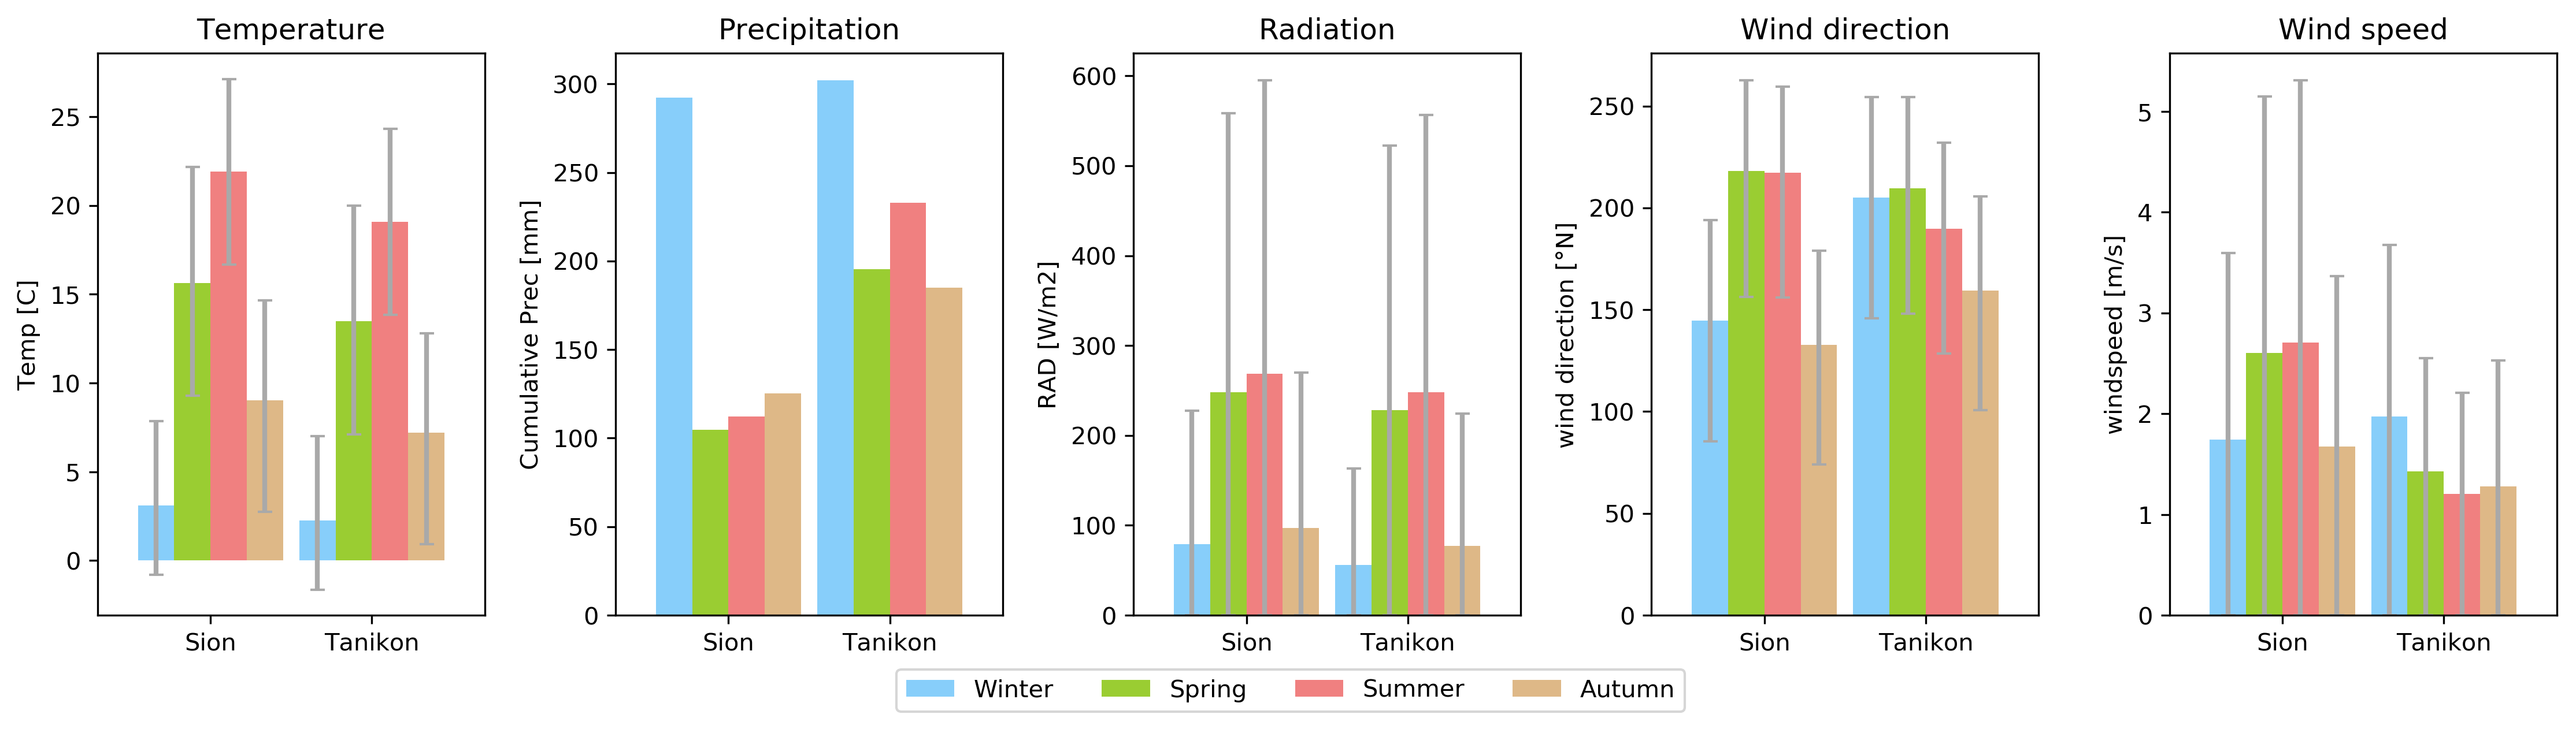
\includegraphics[width = 1 \textwidth]{Figures/season2_avg.png}
        \caption{\textbf{Seasonal changes in meteorological parameters between Sion and Tänikon.} The value displayed for the precipitation is the cumulative sum over the season. The temperature, radiation and wind speed are presented as the mean $\pm$ the standard deviation over the season. Since the wind direction is a periodical entity, its mean and standard deviation is computed in a vectorial fashion.}
        \label{meteo_season}
    \end{figure}
    
    The concentration of air pollutants is highly affected by meteorological parameters such as wind, precipitation, solar radiation or temperature. Presence of wind may carry pollutants away or bring them near the measurement site. It is thus important to take wind into account when trying to understand pollutant emissions. Solar radiation is also a relevant parameter as O\textsubscript{3} is formed indirectly with the help of the solar radiation. Precipitation may capture particulate matter suspended in the air, thus lowering the air concentration of PM10 or PM2.5. Meteorological parameters are not constant in time and location. Consequently, it is important to get insight on the these they vary between Sion and Tänikon on a daily, as well as on a seasonal basis.  The meteorological parameters are summarized in figure \ref{meteo_season}.
    \\
    \\
    The general mean temperature is slightly lower in Tänikon than in Sion. Also the patterns for precipitation are similar, but with higher cumulative value per season in Tänikon. During the spring, summer and autumn, there is approximately 100 mm more seasonal precipitation in Tänikon than in Sion. Sion seems to be sunnier than Tänikon as the radiation per hour is slightly bigger. Note that the values for the solar radiation varies considerably from zero (during) to too very high values during lunchtime. The wind direction is mainly coming from the South-East (150\degree N) and the South-West (200\degree N) at both location while the wind speed seems to be higher in Sion during the spring, summer and autumn than in Tänikon, but a bit higher in winter in Tänikon.
    \\
    In brief, the meteorological parameters (temperature, precipitation, radiation, and wind) present similar patterns between Sion and Tänikon. With the exception, of the higher precipitation in Tänikon during the spring, summer, and autumn. However, they do vary temporally between the seasons. 
    \\
    \\
    By knowing meteorological parameters, it is possible to state some preliminary hypothesis on the evolution of the pollutant concentrations throughout the year (assuming no anthropogenic effects). For example, we expect a high ozone concentration during the spring and the summer since the solar radiation is high . Similarly we expect different concentration between Sion and Tänikon in the spring and the summer since there are on average stronger winds in Sion. 
    \\
    However, the meteorological parameters do not determine the pollutant concentrations all by them-self, because human activities emit many air pollutants. In consequence, the human activity has an influence on the concentrations of air pollutants and the data must be analyzed considering both meteorological and human activity at the same time. 

\section{Monthly evolution} \label{monthly_section}
    % Show the similarities and potential correlation in the monthly average of pollutant
    % -> monthly change between Sion and Tanikon 
    
    \begin{figure}[t]
        \centering
        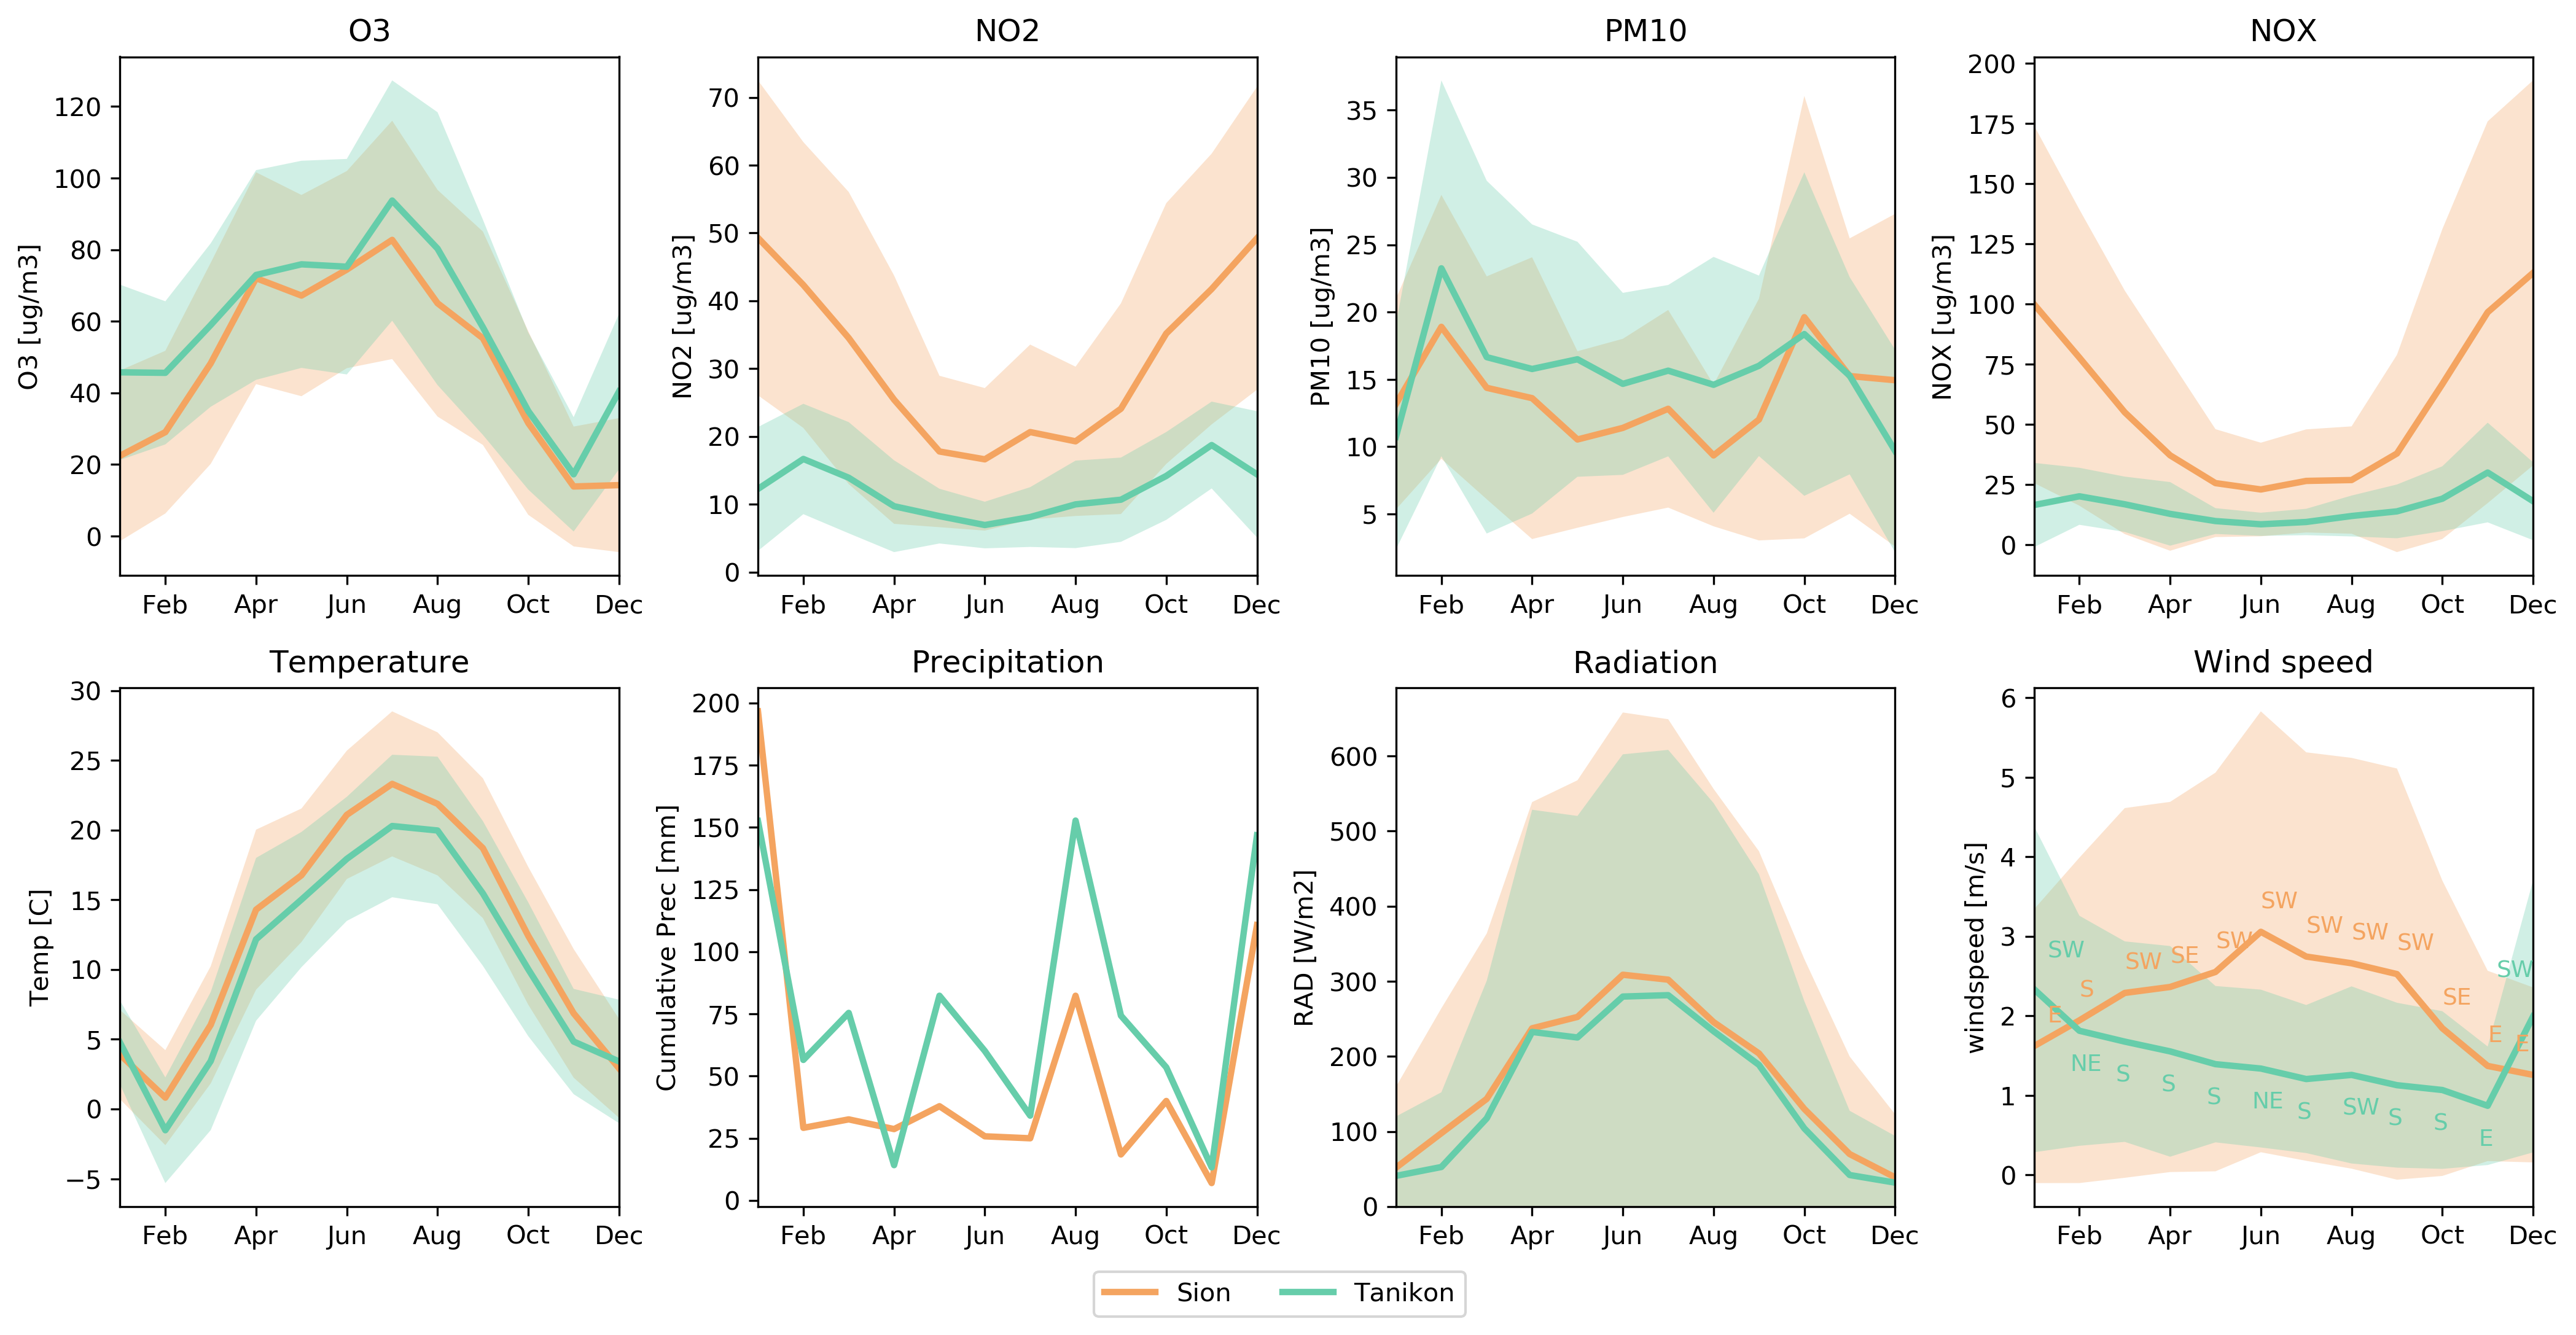
\includegraphics[width = 1 \textwidth]{Figures/monthly_avg2.png}
        \caption{\textbf{Monthly averages of pollutant air concentrations and meteorological parameters.} The value displayed for the precipitation is the cumulative sum over the months. The temperature, radiation, wind speed, O\textsubscript{3}, NO\textsubscript{2}, PM10, and NO\textsubscript{x} are presented as the mean \textpm the standard deviation over the months. The main wind direction is represented on the wind speed plot as a label (N, NE, E, SE, S, SW, W, NW).}
        \label{monthly_evolution}
    \end{figure}
    
    % Describe evolution of pollutants concentrations + meteo param 
    From section \ref{seasonal_section} we can conclude that the meteorological parameters are changing throughout substantially during the year for our two stations. In order to get insight into potential relationships between meteorological parameters and pollutant concentrations, our data was observed for month by month for both Sion and Tänikon. The precipitations was observed as the cumulative rain for each month, whereas the other parameters/concentrations were aggregated by taking their mean for each month. The monthly evolution is presented on figure \ref{monthly_evolution}. 
    \\
    \\
    From the monthly visualization it appears that NO\textsubscript{2} and NO\textsubscript{x} have a similar concentration pattern throughout the year. The concentration is high during the winter months and low during the summer months. However, the concentration for both is much bigger in Sion than in Tänikon. Furthermore, the concentration of NO\textsubscript{x} is consistently higher than the concentration of NO\textsubscript{2}. This confirms the fact that NO\textsubscript{x} is a broader category containing NO\textsubscript{2}. 
    \\
    In contrast to NO\textsubscript{x}, the O\textsubscript{3} concentrations are the highest during the summer months and low during the winter months. The concentrations range approximately from 0 to 120 [\textmu g/m\textsuperscript{3}]. What is more, the concentration of O\textsubscript{3} is more or less the same between Sion and Tänikon. 
    \\
    On the other hand, the mean PM10 concentration appears to be more or less constant through the year at both locations. However, both locations show a slight tendency for higher PM10 concentrations during the winter. In addition, the concentrations for PM10 seem to vary more in Tänikon for the months of February, March and April, while the variation is larger in Sion during the months of October, November and December. 
    \\
    \\
    Finally, a higher radiation as well as a higher temperature is observable in Sion during the summer. The patterns of temperature and radiation are also similar between Sion and Tänikon. In contrast, we observe more rain per month in Tänikon than in Sion, especially during summer.
    \\
    
    \begin{figure}[t]
        \centering
        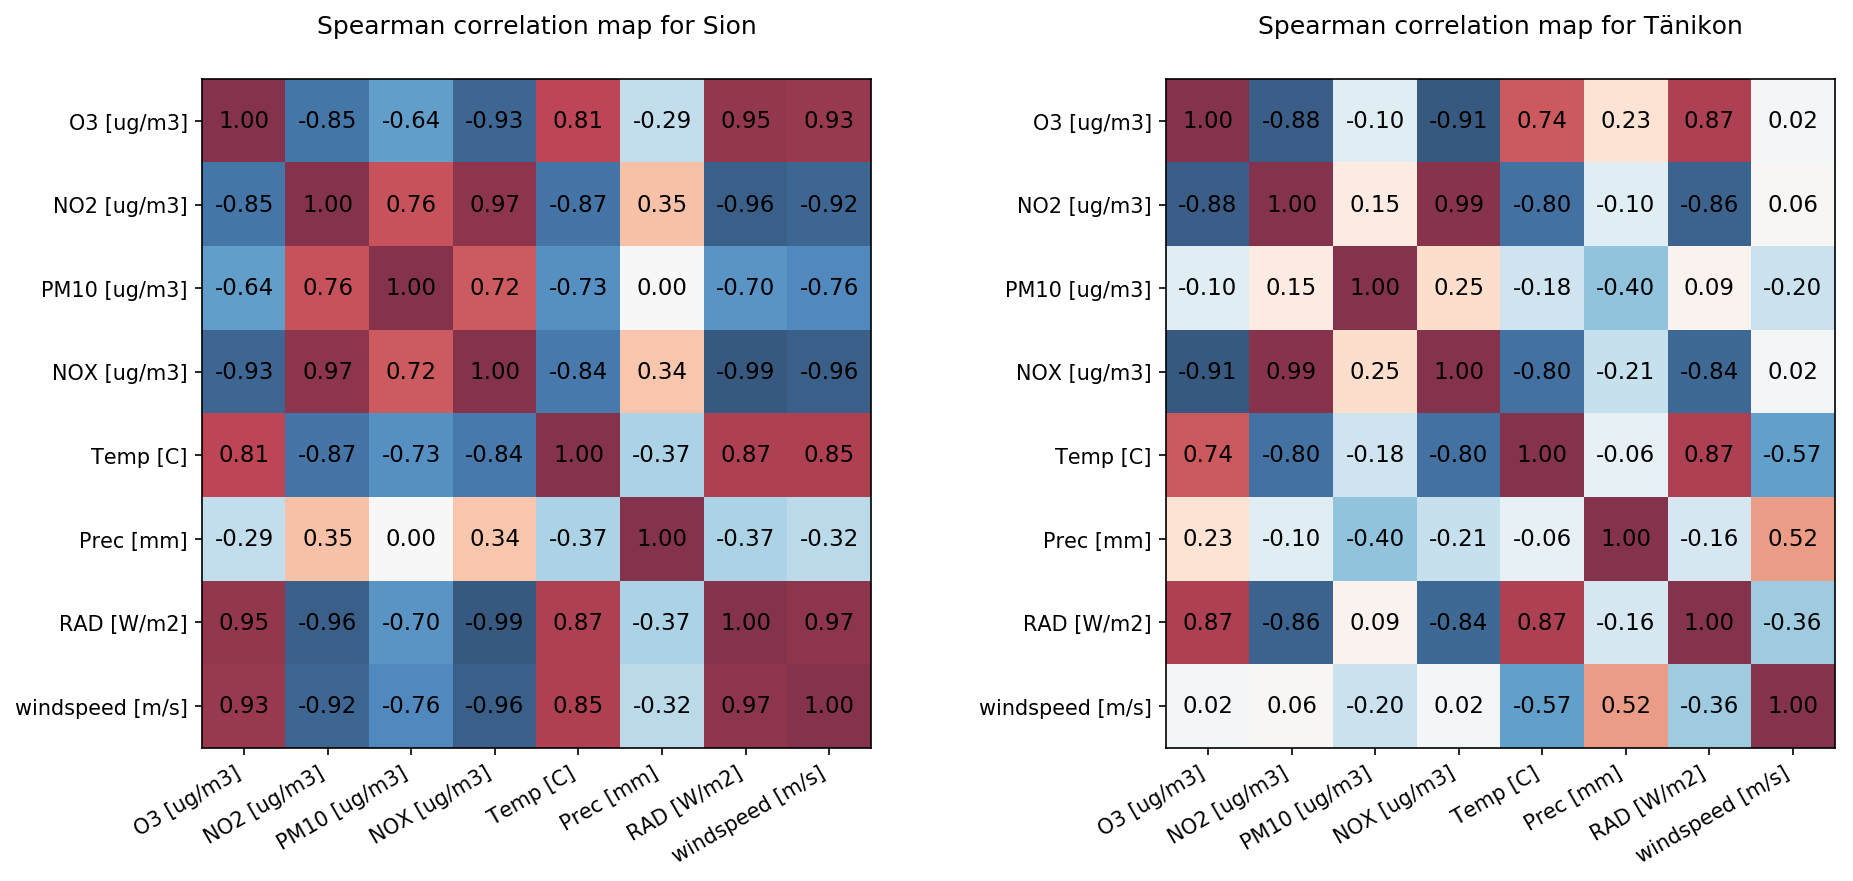
\includegraphics[width = 1 \textwidth]{Figures/monthly_corr.png}
        \caption{\textbf{Spearman correlation map of pollutant air concentrations and meteorological parameters monthly averages.} The spearman coefficient measure how two variables seems to correlate without necessarily being a linear correlation: it estimates how much the two variables can be described as a monotonic function. \\ The spearman coefficients for all of the eight variables is presented in association with a color indicating the correlation (Red corresponds to +1, Blue corresponds to -1, white corresponds to 0)}
        \label{monthly_corr}
    \end{figure}
    
    In order to observe the potential relationships between pollutants and meteorological parameters, the spearman correlation was computed for each pair of variables. The spearman coefficient reflects how well the dependency between two variables can be modeled by a monotonic function. A coefficient of 1 means that the first variable is positively correlated with the second variable, whereas a coefficient of -1 means that the first variable is negatively correlated with the second variable. The obtained coefficients are presented on figure \ref{monthly_corr} as a heat-map: red means a high positive correlation, blue means a high negative correlation, and white means an absence of monotonic correlation.   
    \\
    \\
    First of all, it appears that on both locations, the O\textsubscript{3} is positively correlated with the temperature and the radiation, but is negatively correlated with NO\textsubscript{2} and NO\textsubscript{x}. Inversely, NO\textsubscript{2} and NO\textsubscript{x} are negatively correlated with the temperature and the radiation. This tendency is also observable qualitatively on figure \ref{monthly_evolution}. The observed evolution and dependencies are consistent with the chemical theory that the formation of O\textsubscript{3} relies on solar radiation to 'free' an oxygen from NO\textsubscript{2}. In consequence, O\textsubscript{3} is formed more during the sunny months, namely, April, May, June, July, and August. This confirms the correlation between O\textsubscript{3} and solar radiation. 
    \\ 
    Since NO\textsubscript{2} is necessary for ozone formation, one could expect a positive correlation between the two. However, O\textsubscript{3} may react with NO to produce back NO\textsubscript{2} resulting in a no net production of ozone. Consequently, the amount of O\textsubscript{3} at equilibrium depends on the concentrations NO\textsubscript{2} and the presence of solar radiation. As shown on figure \ref{monthly_evolution}, the concentration of NO\textsubscript{2} (and NO\textsubscript{x}) is higher during winter than during summer. During winter, sunlight is the limiting factor in the formation of ozone, and ozone concentration remains low. During the summer months, there is more sunlight but the concentration of NO\textsubscript{2} drops due to a higher atmospheric mixing layer (new emissions are 'trapped' in a lager volume) and the overall effect is an increase of ozone concentration.
    \\
    \\
    Moreover, on both locations, the cumulative precipitation does not seem to correlate strongly with any other variables. It might be due to the sparsity of the precipitation data and the short term impact of it on the pollutant concentrations. Since most of the data points are measures with zero precipitations (no rain), the monthly average of pollutant concentration is mainly weighted with non-precipitation measures, giving poor credits to this imporant meteorological parameter. 
    \\
    \begin{figure}[t]
        \centering
        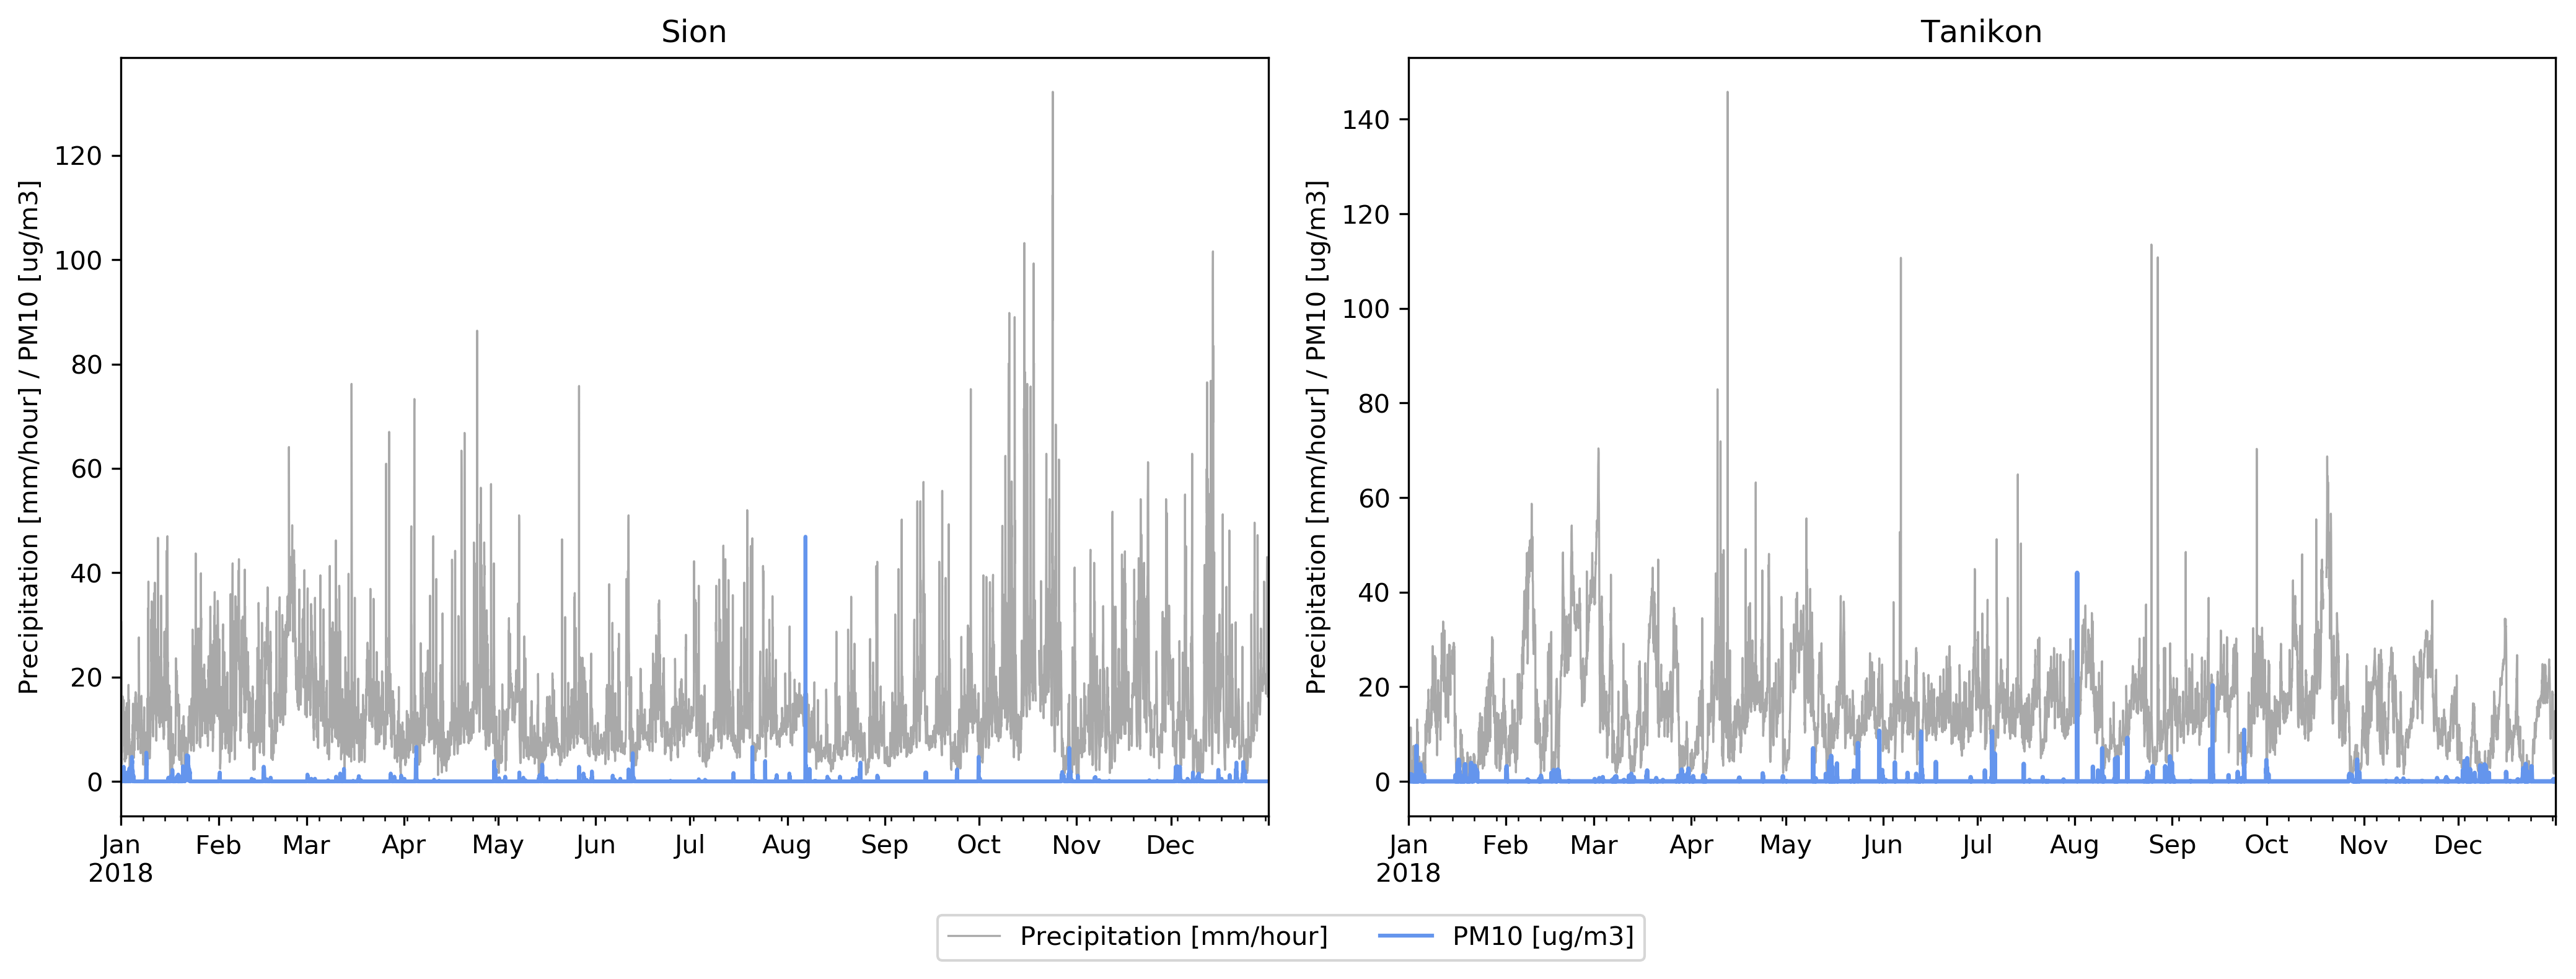
\includegraphics[width = 1 \textwidth]{Figures/Prec_vs_PM10.png}
        \caption{\textbf{PM10 concentration evolution with precipitations.} The hourly measures of PM10 concentration is displayed with the hourly precipitation for both locations. Note that y-scales are not similar since this plot is not used to compare the two locations.}
        \label{PrecvsPM10}
    \end{figure}
    \\
    However, figure \ref{PrecvsPM10} shows that there is a clear relationship between precipitation and PM10 concentration when the hourly values of precipitation are plotted together with the hourly PM10 concentrations. Indeed, whenever there is a rainy event, the PM10 concentration drops, but then increases again when the rain stops. This pattern reflects the fact that rain drops may capture some of the PM10 suspended in the air and bring them down to the ground, thus removing them from the air. This effect seems to be even more visible at the Tänikon station. 
    \\
    \\
    Furthermore, the wind speed correlates differently with the other variables between the two locations. Inn Sion, the wind speed have a strong positive and negative correlation with the other variables, while in Tänikon, the correlation is generally poor. Because of this difference, it is likely that there is a correlation but not especially a causation relationship. It could also be due to the topology as Sion is situated in a valley, but not Tänikon. If there is little wind, the pollutants are trapped in the valley which lead to higher concentration. The concentration is thus much more dependant on the wind in Sion. 
    \\
    \\
    Finally, in Sion the PM10 seems to correlate similarly with other variables as NO\textsubscript{2} (positive correlation with nitrite oxides, and negative correlation with the ozone, temperature, radiation, and wind speed), but with weaker correlations. In Tänikon, PM10 correlates poorly with the other variables. 
    % Causes ? more antropogenic emission ? 
    % Tänikon = countryside -> agriculture ?
    \\
    \\
    In brief, on a monthly basis it seems that the meteorological parameters do influence the pollutant concentrations. For example, a strong solar radiation is a condition for ozone to be formed. Or NO\textsubscript{x} concentrations seem to be influenced by changes in the atmospheric mixing layer. However, the meteorological parameters does not explain all the changes. The NO\textsubscript{2} and NO\textsubscript{x} concentrations are almost systematically higher in Sion than in Tänikon, whereas there are no substantial differences in meteorological parameters between the two locations. Human activity certainly accounts for those differences.
    
\section{Hourly evolution : Weekday vs Weekend}
    
    % to see the effect of human activity --> look at week end week day (no change in meteo)
    The pollutant concentrations are dependent on meteorological parameters that change over the year. In consequence it is hard to differentiate the changes of concentration due to meteorological variations from the changes due to human activities. That is why the average diurnal evolution is studied separately on week and week-end days for both Sion and Tänikon. The meteorological parameters should not depend on weekday/week-end day distinction since it's a human concept. The human activity however changes between weekday and week-end days. Figure \ref{daily_evolution} presents the average diurnal concentrations for weekday and week-end days in both Sion and Tänikon.
    \\
    \\
    First of all, the eight bottom plots of figure \ref{daily_evolution} present the meteorological parameters for both locations between weekday and week-end days. They enable to check that they do not change on average between the type of day. This is however the case at both locations since both curves overlap almost perfectly. Only the precipitation is different between weekday and week-end days. It's higher during the weekdays because the precipitations are aggregated as a cumulative sum over the week (or week-end) days and as a consequence, the weekday diurnal precipitation is the sum over 2.5 more days than the week-end days, resulting in a higher cumulative sum. 
    \\
    \begin{figure}[!t]
        \centering
        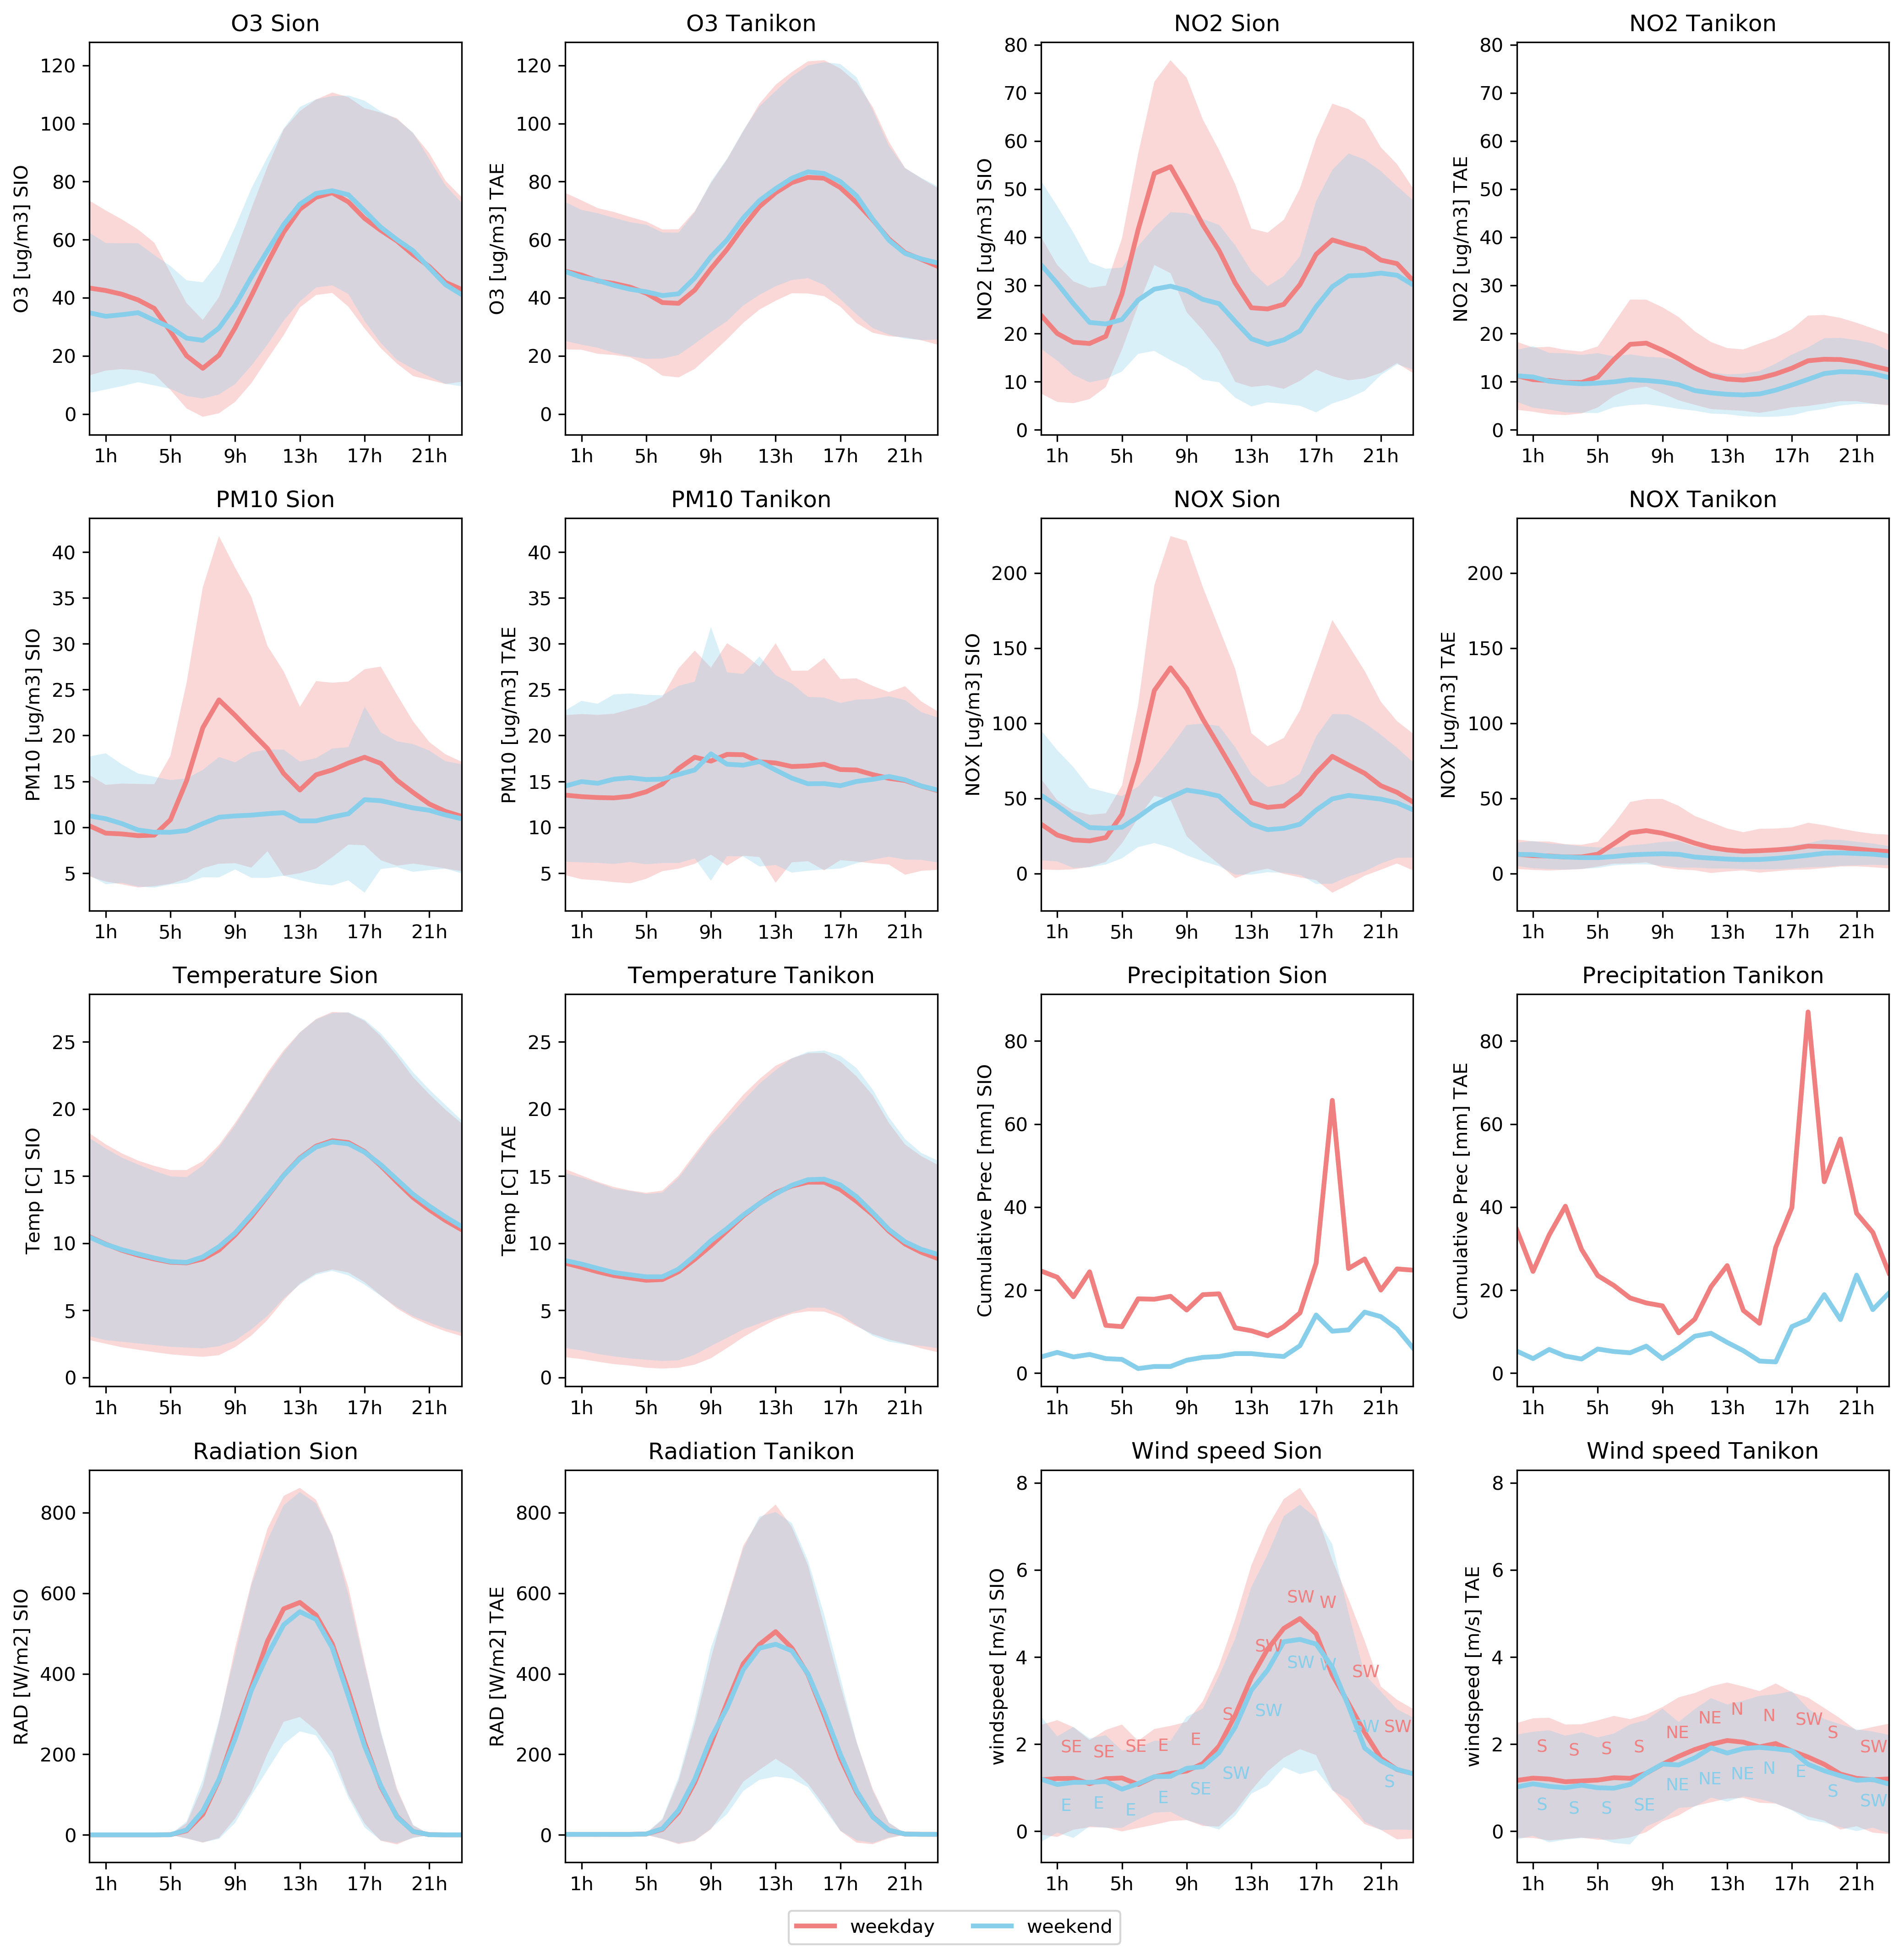
\includegraphics[width = 1 \textwidth]{Figures/daily_avg.png}
        \caption{\textbf{Hourly averages of air pollutant concentrations and meteorological parameters for weekdays and weekend days.} The value displayed for the precipitation is the cumulative sum over the hours of the day. The temperature, radiation, wind speed, O\textsubscript{3}, NO\textsubscript{2}, PM10, and NO\textsubscript{x} are presented as the mean \textpm the standard deviation over the hours of the day. The main wind direction is represented on the wind speed plot as a label (N, NE, E, SE, S, SW, W, NW). Note that each plot displaying similar parameter (for Sion (SIO) and Tänikon(TAE)) have the same y scale to enable comparison}
        \label{daily_evolution}
    \end{figure}
    \\
    On both locations the O\textsubscript{3} concentration appears to be similar between the weekdays and week-end days. The only notable difference is happening in Sion around 8 o'clock, where the concentration gets lower in week days (the same effect is slightly visible on the Tänikon plot). The independence of ozone from week/week-end distinction may suggest that the human activities does not have on strong effect on its concentration and that it's mainly influenced by weather parameters. The diurnal data are consistent with the importance of solar radiation for O\textsubscript{3} formation. Indeed, the sun rises between 6 and 9 o'clock and at this time, the ozone concentration is increasing until 17 o'clock which represent the time where the the solar radiation weakens before the sun sets. \\
    The difference between weekdays and week-end days in Sion (and Tänikon) around 8 o'clock may be due to the traffic of people going to work. Internal combustion car engines (especially Diesel) produce NO\textsubscript{x} and under the hypothesis of a rather low VOC (volatile organic compounds) in the morning \footnote{The measurement stations are not in forest or near a gasoline station which are considered high VOC areas.}, a decrease of ozone would be present at high NO\textsubscript{x}. However, as traffic increases and as the sun rises, the NO\textsubscript{x} as well as VOC increases (produced by cars) which leads to increasing O\textsubscript{3} concentrations.
    \\
    \\
    The NO\textsubscript{2}, NO\textsubscript{x} and PM10 concentrations show similar patterns in Sion during the weekdays. The three of them show a substantial increase between 5 and 9 o'clock and a decrease until 13-14 o'clock as well as a second increase between 15-18 o'clock. This pattern seems to correspond with the high traffic pattern: in the morning to go to work and on the evening to go back home. This hypothesis is consistent with the emissions observed. Indeed, the heat in cars engines catalyzes NO\textsubscript{2} and NO\textsubscript{x} formation, while the car exhausts release many incompletely burned compounds generating PM10. In consequence, the  more cars on the roads, the more emissions we can observe. This pattern is attenuated during week-end days and the difference can be attributed to the decreased human activity during the week-end days. 
    \\
    A similar pattern is observable in Tänikon for NO\textsubscript{2} and NO\textsubscript{x}, but in a more attenuated fashion (roughly four times less). However the PM10 concentration does not follow the same pattern between Sion and Tänikon and appears to be approximately constant (around 15 [\textmu g/m\textsubscript{3}]) with no clear differences between week and week-end days. This higher constant PM10 concentration in Tänikon than in Sion can potentially be due to the countryside nature of the measurement station localization. Tänikon is a village surrounded by crops and the measurement station is placed in the middle of a crop. In consequence, a lot of dust might be stirred up by the wind, thus increasing the PM10 concentration. There might also be some particulate matter produced during the harvesting periods. Hence, the PM10 concentration would be less dependant on human weekday activities, and the concentration would be similar between week and week-end days. 
    \\
    \\
    In brief, observing the diurnal evolution between week and week-end days allows to highlight the human effect on the concentrations of air pollutants. As expected, the weather parameters are similar for week and week-end days. It also appears that O\textsubscript{3} is roughly similar during the week, suggesting that human activities does not impact much the ozone concentrations. On the other hand, the NO\textsubscript{2} and NO\textsubscript{x} concentrations show a clear difference between week and week-end days which is consistent with the high traffic period (morning and evening rush hours). The difference is stronger in Sion than in Tänikon, certainly because of the environment in which the measure station is placed : near the highway in Sion and in the countryside in Tänikon. 
    
\section{Legal limits exceeding}
    % Present what are the legal limits in Switzerland and to which pollutants they apply
    % Describe the table 1 and how the limits are or not overpassed
    % constrast between both locations : Same polluatnt overpassing ? overpassing at the same period of the year ? how big is the overpassing ?
        
    \begin{table}[t]
        \caption{\textbf{Legal limit exceedance.} The legal emission limits are presented for each of the regulated pollutant measured, namely PM10, NO\textsubscript{2}, and O\textsubscript{3}. The \textit{Exceeded} column states if the limit has been exceeded. For 24h averages and hourly averages, the number of continuous period in which the limit has been exceeded is reported as well as the number of hours those periods represents. Note that the number of hours represents the number of hour in which the average over the 24 preceding hours exceed the limit. For annual average, the \textit{deviation from the limit} is provided, it represents from how much the limit has or not been exceeded.}
        \label{table_legal}
        \resizebox{\textwidth}{!}{%
        \begin{tabular}{@{}cccccccccc@{}}
        \toprule
                              &                & \multicolumn{4}{c}{Sion}                                  & \multicolumn{4}{c}{Tänikon}                               \\ \midrule
                              &                & Exceeded & Nbr periods & Nbr hours & deviation from limit & Exceeded & Nbr periods & Nbr hours & deviation from limit \\ \midrule
        \multirow{2}{*}{PM10} & 24h average    & NO       & 0           & 0         & -                    & YES      & 2           & 39        & -                    \\
                              & annual average & NO       & -           & -         & -6.22 [\textmu g/m\textsuperscript{3}]         & NO       & -           & -         & -4.46 [\textmu g/m\textsuperscript{3}]         \\ \midrule
        \multirow{2}{*}{NO\textsubscript{2}}  & 24h average    & YES      & 1           & 11        & -                    & NO       & 0           & 0         & -                    \\
                              & annual average & YES      & -           & -         & 1.30 [\textmu g/m\textsuperscript{3}]          & NO       & -           & -         & -18.03 [\textmu g/m\textsuperscript{3}]        \\ \midrule
        O\textsubscript{3}                    & hourly average & YES      & 55          & 193       & -                    & YES      & 85          & 489       & -                    \\ \bottomrule
        \end{tabular}%
        }
    \end{table}
    
    Air pollutants such as NO\textsubscript{2}, NO\textsubscript{x}, O\textsubscript{3} and PM10 can have a negative impact on human health. NO\textsubscript{2} may irritates airways and induce respiratory difficulties \cite{NO2Health}. O\textsubscript{3} also induces airways irritation and increase respiratory infections risks \cite{OzoneHealth}. PM10 are small enough to travel deep in the lung to reach the alveolus where they can potentially enter the blood stream. Hence, they may cause lung functions reductions and an increased risk of heart attacks \cite{PM10Health}. In addition, these pollutant have also an environmental impact. NO\textsubscript{2} increases acidic rain and participates in the formation of winter smog. PM10 also increases acidity of lakes and streams. 
    \\
    \begin{figure}[!t]
        \centering
        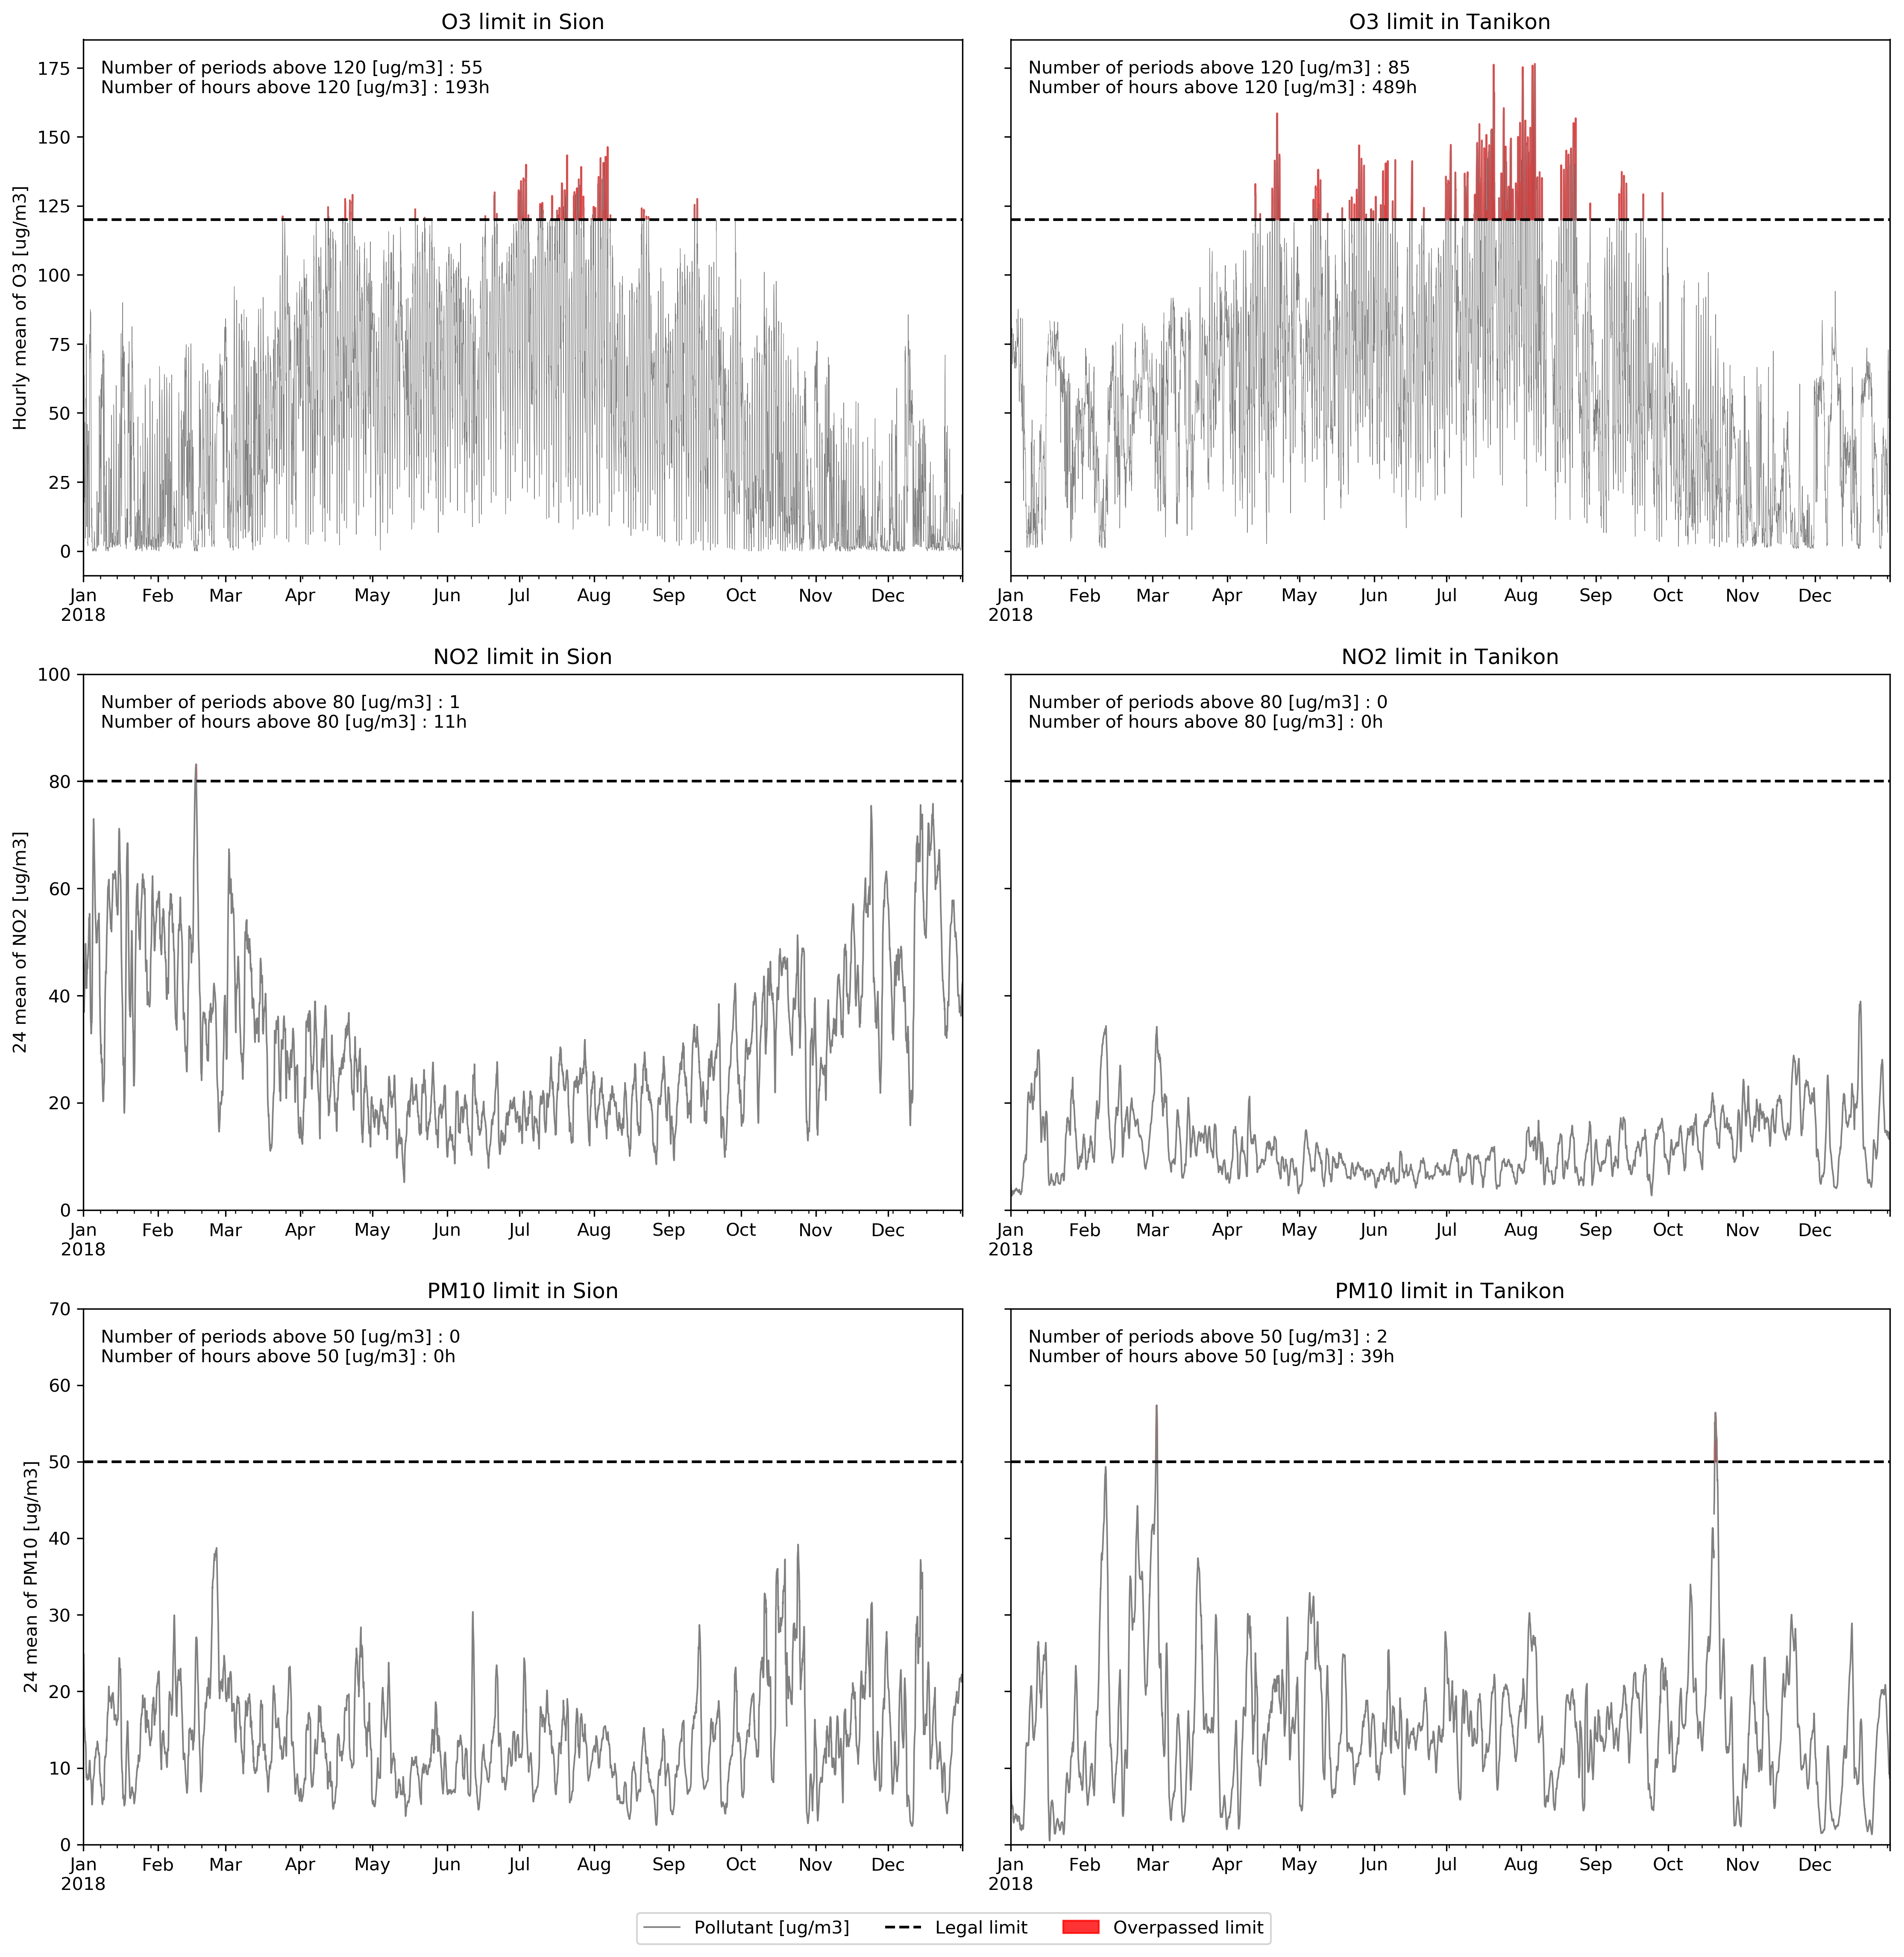
\includegraphics[width = 1 \textwidth]{Figures/limit.png}
        \caption{\textbf{O\textsubscript{3}, NO\textsubscript{2} and PM10 legal limitations exceedance for both Sion and Tänikon} The concentrations of the air pollutants are displayed together with the associated legal limits. The red area shows when the concentration of pollutant exceeds the legal limit. For ozone, the hourly concentration is visualized, while for NO\textsubscript{2} and PM10 the 24h average is shown. The text annotations on the plot define the number of different periods where the legal limit is exceeded. It also report the number of hour it represents.}
        \label{legal_limit}
    \end{figure}
    Due to these negative consequences of air pollutants, legal regulation has been imposed on the studied pollutants in Switzerland. The hourly average ozone concentration should not exceed 120 [\textmu g/m\textsubscript{3}] through the year. The average concentration of NO\textsubscript{2} over a 24h period should not exceed 80 [\textmu g/m\textsubscript{3}] and the annual average NO\textsubscript{2} concentration must not exceed 30 [\textmu g/m\textsubscript{3}]. The average concentration of PM10 over 24h periods should not exceed 50 [\textmu g/m\textsubscript{3}] and the annual average PM10 concentration must not exceed 20 [\textmu g/m\textsubscript{3}]. There are no regulations directly on NO\textsubscript{x} concentrations, but only on NO\textsubscript{2}. There are half-hour regulations on NO\textsubscript{2} and O\textsubscript{3} as well (respectively 95\% and 98\% of half-hour average concentrations should not exceed 100 [\textmu g/m\textsubscript{3}]). However, these special limits could not be assessed as the available data has a temporal resolution of an hour. 
    \\
    \\
    Table \ref{table_legal} summarizes the legal regulations for NO\textsubscript{2}, O\textsubscript{3}, and PM10, in both Sion and Tänikon. This table also presents the amount of periods/hours during which the limit has been exceeded. For the annual mean, the difference between the limit and the actual mean is also presented. Figure \ref{legal_limit}, shows the concentration over time with highlighted exceedances.
    \\
    \\
    First of all, it appears from table \ref{table_legal} that the ozone hourly concentration limit has been exceeded multiple times during the year 2018 both in Sion and Tänikon. The exceedance is larger in Tänikon than in Sion. In addition, Figure \ref{legal_limit} shows at which time of the year those exceedances occurs. They all occurred between April and October and concentrate in the period between July and August. This makes sense as ozone formation requires solar radiation which is at its strongest during these months. 
    \\
    \\
    Secondly, the 24h average PM10 concentrations exceeds the limit only in Tänikon during 2 periods. These periods of exceedance display a spiking behavior: the concentration is almost two times larger than the usual. It thus seems that the exceedance is due an irregular event. Those two exceedance periods occurs around the beginnings of March 2018 and around the 20th of October. The high concentration in PM10 between the end of February and the beginning of March matches with a period a cold temperature in Tänikon during which people of the village have certainly had to increase the heating of their house. It is likely that a part of those house relies on an old combustion system for heating (like wood). Such heating would increase the PM10 concentration. \\
    On both locations the annual means stays below the legal limit. The annual means represents approximately 75\% of the limit, it is thus way below it. 
    \\
    \\
     On the other hand, the 24h average of NO\textsubscript{2} concentrations exceeds the limits only in Sion and only once, around mid-February. This exceedance also presents a spiking behavior. This spike corresponds roughly with the carnival in Valais (around the 13 of February) and many people may have been using fireworks and used their car to drive from/to the carnival. As observed in section \ref{monthly_section}, the NO\textsubscript{2} concentration is higher during the winter and the concentration is close to the limit but still below with some margin. Moreover, the annual concentration of NO\textsubscript{2} is exceeded only in Sion but only by 4\% of the limit. 
    
\section{Conclusion}
    The descriptive analysis of this work has explored the impact of meteorological parameters (Temperature, radiation, precipitation and wind) on O\textsubscript{3}, NO\textsubscript{2}, NO\textsubscript{2}, and PM10. We can draw the following two conclusions from our data: The ozone concentration depends strongly on solar radiation and the PM10 concentration drops substantially after a day of rain. The concentrations of these two pollutants is thus heavily influenced by weather conditions. However, also an anthropogenic impact has been observed: We can conclude that the concentration of NO\textsubscript{2} and NO\textsubscript{x} is increased during week days during the rush hours (6-9 o'clock and 15-18 o'clock), while the concentrations are considerably lower during the weekend (when less cars circulate). The anthropogenic is stronger at the Sion measurement station as it in the immediate vicinity of to the highway A9. Finally, the exceedance of legal limits for several pollutants has been observed. While most pollutants stay within the legal boundaries most of the time, Ozone is consistently exceeding its legal limit during most of the summer. Furthermore, there are few punctual events during which the concentrations of NO\textsubscript{2} and PM10 exceed the limits, however the amount of excess is generally small and limited to a short time period.

\newpage
\bibliographystyle{unsrt}
\bibliography{references}

\end{document}